% Options for packages loaded elsewhere
% Options for packages loaded elsewhere
\PassOptionsToPackage{unicode}{hyperref}
\PassOptionsToPackage{hyphens}{url}
\PassOptionsToPackage{dvipsnames,svgnames,x11names}{xcolor}
%
\documentclass[
  12pt,
  letterpaper,
  DIV=11,
  numbers=noendperiod]{scrartcl}
\usepackage{xcolor}
\usepackage{amsmath,amssymb}
\setcounter{secnumdepth}{5}
\usepackage{iftex}
\ifPDFTeX
  \usepackage[T1]{fontenc}
  \usepackage[utf8]{inputenc}
  \usepackage{textcomp} % provide euro and other symbols
\else % if luatex or xetex
  \usepackage{unicode-math} % this also loads fontspec
  \defaultfontfeatures{Scale=MatchLowercase}
  \defaultfontfeatures[\rmfamily]{Ligatures=TeX,Scale=1}
\fi
\usepackage{lmodern}
\ifPDFTeX\else
  % xetex/luatex font selection
  \setmainfont[]{Times New Roman}
\fi
% Use upquote if available, for straight quotes in verbatim environments
\IfFileExists{upquote.sty}{\usepackage{upquote}}{}
\IfFileExists{microtype.sty}{% use microtype if available
  \usepackage[]{microtype}
  \UseMicrotypeSet[protrusion]{basicmath} % disable protrusion for tt fonts
}{}
\makeatletter
\@ifundefined{KOMAClassName}{% if non-KOMA class
  \IfFileExists{parskip.sty}{%
    \usepackage{parskip}
  }{% else
    \setlength{\parindent}{0pt}
    \setlength{\parskip}{6pt plus 2pt minus 1pt}}
}{% if KOMA class
  \KOMAoptions{parskip=half}}
\makeatother
% Make \paragraph and \subparagraph free-standing
\makeatletter
\ifx\paragraph\undefined\else
  \let\oldparagraph\paragraph
  \renewcommand{\paragraph}{
    \@ifstar
      \xxxParagraphStar
      \xxxParagraphNoStar
  }
  \newcommand{\xxxParagraphStar}[1]{\oldparagraph*{#1}\mbox{}}
  \newcommand{\xxxParagraphNoStar}[1]{\oldparagraph{#1}\mbox{}}
\fi
\ifx\subparagraph\undefined\else
  \let\oldsubparagraph\subparagraph
  \renewcommand{\subparagraph}{
    \@ifstar
      \xxxSubParagraphStar
      \xxxSubParagraphNoStar
  }
  \newcommand{\xxxSubParagraphStar}[1]{\oldsubparagraph*{#1}\mbox{}}
  \newcommand{\xxxSubParagraphNoStar}[1]{\oldsubparagraph{#1}\mbox{}}
\fi
\makeatother


\usepackage{longtable,booktabs,array}
\usepackage{calc} % for calculating minipage widths
% Correct order of tables after \paragraph or \subparagraph
\usepackage{etoolbox}
\makeatletter
\patchcmd\longtable{\par}{\if@noskipsec\mbox{}\fi\par}{}{}
\makeatother
% Allow footnotes in longtable head/foot
\IfFileExists{footnotehyper.sty}{\usepackage{footnotehyper}}{\usepackage{footnote}}
\makesavenoteenv{longtable}
\usepackage{graphicx}
\makeatletter
\newsavebox\pandoc@box
\newcommand*\pandocbounded[1]{% scales image to fit in text height/width
  \sbox\pandoc@box{#1}%
  \Gscale@div\@tempa{\textheight}{\dimexpr\ht\pandoc@box+\dp\pandoc@box\relax}%
  \Gscale@div\@tempb{\linewidth}{\wd\pandoc@box}%
  \ifdim\@tempb\p@<\@tempa\p@\let\@tempa\@tempb\fi% select the smaller of both
  \ifdim\@tempa\p@<\p@\scalebox{\@tempa}{\usebox\pandoc@box}%
  \else\usebox{\pandoc@box}%
  \fi%
}
% Set default figure placement to htbp
\def\fps@figure{htbp}
\makeatother


% definitions for citeproc citations
\NewDocumentCommand\citeproctext{}{}
\NewDocumentCommand\citeproc{mm}{%
  \begingroup\def\citeproctext{#2}\cite{#1}\endgroup}
\makeatletter
 % allow citations to break across lines
 \let\@cite@ofmt\@firstofone
 % avoid brackets around text for \cite:
 \def\@biblabel#1{}
 \def\@cite#1#2{{#1\if@tempswa , #2\fi}}
\makeatother
\newlength{\cslhangindent}
\setlength{\cslhangindent}{1.5em}
\newlength{\csllabelwidth}
\setlength{\csllabelwidth}{3em}
\newenvironment{CSLReferences}[2] % #1 hanging-indent, #2 entry-spacing
 {\begin{list}{}{%
  \setlength{\itemindent}{0pt}
  \setlength{\leftmargin}{0pt}
  \setlength{\parsep}{0pt}
  % turn on hanging indent if param 1 is 1
  \ifodd #1
   \setlength{\leftmargin}{\cslhangindent}
   \setlength{\itemindent}{-1\cslhangindent}
  \fi
  % set entry spacing
  \setlength{\itemsep}{#2\baselineskip}}}
 {\end{list}}
\usepackage{calc}
\newcommand{\CSLBlock}[1]{\hfill\break\parbox[t]{\linewidth}{\strut\ignorespaces#1\strut}}
\newcommand{\CSLLeftMargin}[1]{\parbox[t]{\csllabelwidth}{\strut#1\strut}}
\newcommand{\CSLRightInline}[1]{\parbox[t]{\linewidth - \csllabelwidth}{\strut#1\strut}}
\newcommand{\CSLIndent}[1]{\hspace{\cslhangindent}#1}



\setlength{\emergencystretch}{3em} % prevent overfull lines

\providecommand{\tightlist}{%
  \setlength{\itemsep}{0pt}\setlength{\parskip}{0pt}}



 


\usepackage{tcolorbox}
\usepackage{amssymb}
\usepackage{yfonts}
\usepackage{bm}


\newtcolorbox{greybox}{
  colback=white,
  colframe=blue,
  coltext=black,
  boxsep=5pt,
  arc=4pt}
  
\newcommand{\sectionbreak}{\clearpage}

 
\newcommand{\ds}[4]{\sum_{{#1}=1}^{#3}\sum_{{#2}=1}^{#4}}
\newcommand{\us}[3]{\mathop{\sum\sum}_{1\leq{#2}<{#1}\leq{#3}}}

\newcommand{\ol}[1]{\overline{#1}}
\newcommand{\ul}[1]{\underline{#1}}

\newcommand{\amin}[1]{\mathop{\text{argmin}}_{#1}}
\newcommand{\amax}[1]{\mathop{\text{argmax}}_{#1}}

\newcommand{\ci}{\perp\!\!\!\perp}

\newcommand{\mc}[1]{\mathcal{#1}}
\newcommand{\mb}[1]{\mathbb{#1}}
\newcommand{\mf}[1]{\mathfrak{#1}}

\newcommand{\eps}{\epsilon}
\newcommand{\lbd}{\lambda}
\newcommand{\alp}{\alpha}
\newcommand{\df}{=:}
\newcommand{\am}[1]{\mathop{\text{argmin}}_{#1}}
\newcommand{\ls}[2]{\mathop{\sum\sum}_{#1}^{#2}}
\newcommand{\ijs}{\mathop{\sum\sum}_{1\leq i<j\leq n}}
\newcommand{\jis}{\mathop{\sum\sum}_{1\leq j<i\leq n}}
\newcommand{\sij}{\sum_{i=1}^n\sum_{j=1}^n}
	
\KOMAoption{captions}{tableheading}
\makeatletter
\@ifpackageloaded{caption}{}{\usepackage{caption}}
\AtBeginDocument{%
\ifdefined\contentsname
  \renewcommand*\contentsname{Table of contents}
\else
  \newcommand\contentsname{Table of contents}
\fi
\ifdefined\listfigurename
  \renewcommand*\listfigurename{List of Figures}
\else
  \newcommand\listfigurename{List of Figures}
\fi
\ifdefined\listtablename
  \renewcommand*\listtablename{List of Tables}
\else
  \newcommand\listtablename{List of Tables}
\fi
\ifdefined\figurename
  \renewcommand*\figurename{Figure}
\else
  \newcommand\figurename{Figure}
\fi
\ifdefined\tablename
  \renewcommand*\tablename{Table}
\else
  \newcommand\tablename{Table}
\fi
}
\@ifpackageloaded{float}{}{\usepackage{float}}
\floatstyle{ruled}
\@ifundefined{c@chapter}{\newfloat{codelisting}{h}{lop}}{\newfloat{codelisting}{h}{lop}[chapter]}
\floatname{codelisting}{Listing}
\newcommand*\listoflistings{\listof{codelisting}{List of Listings}}
\makeatother
\makeatletter
\makeatother
\makeatletter
\@ifpackageloaded{caption}{}{\usepackage{caption}}
\@ifpackageloaded{subcaption}{}{\usepackage{subcaption}}
\makeatother
\usepackage{bookmark}
\IfFileExists{xurl.sty}{\usepackage{xurl}}{} % add URL line breaks if available
\urlstyle{same}
\hypersetup{
  pdftitle={Nonmetric Strain},
  pdfauthor={Jan de Leeuw},
  colorlinks=true,
  linkcolor={blue},
  filecolor={Maroon},
  citecolor={Blue},
  urlcolor={Blue},
  pdfcreator={LaTeX via pandoc}}


\title{Nonmetric Strain}
\author{Jan de Leeuw}
\date{March 6, 2026}
\begin{document}
\maketitle
\begin{abstract}
The three major loss functions for multidimensional scaling, in order of
decreasing popularity, are stress, sstress, and strain. The strain loss
function has been applied mostly in classical metric MDS of complete
distances matrices, although some extensions to additive constants,
bound constraints, missing data, and ordinal scaling have been discussed
in the literature. We use alternating least squares (ALS) and
majorization (MM) to develop various forms of non-metric MDS based on
strain minimization, together with corresponding programs in R.
\end{abstract}

\renewcommand*\contentsname{Table of contents}
{
\hypersetup{linkcolor=}
\setcounter{tocdepth}{3}
\tableofcontents
}

\sectionbreak

\textbf{Note:} This is a working manuscript which will be
expanded/updated frequently. All suggestions for improvement are
welcome. All Rmd, tex, html, pdf, R, and C files are in the public
domain. Attribution will be appreciated, but is not required. The files
can be found at \url{https://github.com/deleeuw/strain}

\sectionbreak

\section{Introduction}\label{introduction}

In Mutidimensional Scaling (MDS) the strain loss function is defined as
\begin{equation}
\sigma(X,\Delta):=\frac14\text{tr}\ \{J(\Delta^2-D^2(X))J\}^2\label{eq-strain}
\end{equation} Here \(J\) is the centering matrix of order \(n\),
i.e.~\(J:=I-n^{-1}E\), with \(E\) a matrix with all elements equal to
one. Matrix \(\Delta^2\) has squared dissimilarities and \(D^2(X)\)
contains the squared Euclidean distances between the rows of an
\(n\times p\) column-centered configuration matrix \(X\).

We will also use another representation of strain in this paper. By
applying the classical embedding result of Schoenberg
(\citeproc{ref-schoenberg_35}{1935}) and Young and Householder
(\citeproc{ref-young_householder_38}{1938}), in the version proposed by
Torgerson (\citeproc{ref-torgerson_58}{1958}), we find \begin{equation}
\sigma(X,\Delta)=\text{tr}\ (C- XX')^2.\label{eq-strainc}
\end{equation} with \begin{equation}
C:=-\frac12 J\Delta^2J.\label{eq-c}
\end{equation}

In \emph{metric} MDS the matrix \(\Delta\) is constant and given, and we
minimize strain over \(X\). From \eqref{eq-strainc} the basic theorem of
Classical Scaling (Torgerson (\citeproc{ref-torgerson_58}{1958})), also
known as Principal Coordinate Analysis (Gower
(\citeproc{ref-gower_66}{1966})), tells us that the optimal \(X\) are
the eigenvectors corresponding with the \(p\) largest eigenvalues of
\(C_+\), the positive definite part of \(C\), with each eigenvector
scaled to have norm equal to the square root of the corresponding
eigenvalue There are rigorous proofs in Keller
(\citeproc{ref-keller_62}{1962}) and De Leeuw
(\citeproc{ref-deleeuw_R_74c}{1974a}).

In non-metric MDS we have to minimize strain over both \(X\) and
\(\Delta\), where \(\Delta\) varies in some subset of the space
\(\mathfrak{D}\) of non-negative, symmetric and hollow matrices of order
\(n\). Classical examples, treated in detail in this paper, are the
additive constant problem, the missing data problem, the use of bound
constraints, and ordinal non-metric scaling.

The history of various tentative and/or incomplete attempts to construct
a non-metric MDS technique based on strain is in De Leeuw and Heiser
(\citeproc{ref-deleeuw_heiser_C_82}{1982}) and Trosset
(\citeproc{ref-trosset_98}{1998}). The first systematic approach to the
problem is in De Leeuw (\citeproc{ref-deleeuw_R_74b}{1974b}), who
discusses the additive constant problem, the missing data problem, and
the ordinal forms of MDS. There is not software in De Leeuw
(\citeproc{ref-deleeuw_R_74b}{1974b}), only equations. The paper
proposes a minimization approach based on what Trosset
(\citeproc{ref-trosset_97}{1997}) calls ``variable reduction''. The
minimum of strain over \(X\), which equals the sum of squares of the
discarded eigenvalues of \(C_+\), is minimized over \(\Delta\). Results
from classical perturbation theory are used to give expression for the
first and second derivatives of this ``reduced'' loss function, with the
implicit understanding that these derivatives can be used in a large
variety of general-purpose optimization methods.

An early implementation of the same methodology for the additive
constant problem is in Saito (\citeproc{ref-saito_78}{1978}). Since the
``reduced'' strain in that case only depends on a single parameter (the
additive constant) Saito uses a simple bisection-type search procedure
on the positive real line for minimization.

The a multi-parameter non-metric scaling problem occurs when some of the
\(\delta_{ij}\) are missing, either by accident or by design. Thus
\begin{equation}
\delta_{ij}=\begin{cases}\delta_{ij}^0&\text{ for non-missing},\\
\theta_{ij}&\text{ for missing}.
\end{cases}
\end{equation} Thus the number of additional parameters is equal to the
number of missing elements. We will require the \(\theta_{ij}\) to be
non-negative. An important special case of the missing data problem is
the unfolding problem, in which we have similarities between objects in
two disjoint sets. The between-set distances are known, while both
matrices of within-set distances are missing.

A third important form of non-metric MDS is ordinal MDS. We require the
\(\delta_{ij}\) to non-negative and monotone with the \(\delta_{ij}^0\).
More precisely if \(\delta_{ij}^0\geq\delta_{kl}^0\) then we must have
\(\delta_{ij}\geq\delta_{kl}\geq 0\).

A systematic and general approach, similar to but much more detailed
than De Leeuw (\citeproc{ref-deleeuw_R_74b}{1974b}), was followed by
Michael Trosset in a sequence of papers (Trosset
(\citeproc{ref-trosset_97}{1997}), Trosset
(\citeproc{ref-trosset_00}{2000}), Trosset
(\citeproc{ref-trosset_98}{1998}), Trosset
(\citeproc{ref-trosset_02}{2002})). Trosset addresses the additive
constant problem, bound constraints, the missing data problem (as a
special case of bound constraints), and ordinal MDS. He also compares
variable reduction methods with ``variable alternation'' methods, which
iteratively alternate minimization over \(X\) with minimization over
\(\Delta\). For the variable reduction methods, which he favors, he
relies on established general purpose mathematical programming routines
to minimize the reduced loss function.

In this paper we use a methodology which differs from Trosset's in two
important respects. We propose and implement variable alternation
methods instead of variable reduction methods, and we use majorization
(MM) to minimize over \(X\). This produces a class of flexible
techniques with monotone convergence and relatively small storage
requirements that can be adapted easily to alternative constraints on
\(X\) and/or \(\Delta\). We have no actual comparisons, but theoretical
considerations suggest that specialized variable reduction techniques
can be made to converge faster than variable alternation techniques.
This depends on the well-known trade-off between the number of
iterations required for convergence and the amount of computation in a
single iteration.

\sectionbreak

\section{Alternating Least Squares}\label{alternating-least-squares}

In our technique for strain minimization we apply alternating least
squares (ALS) to loss function \eqref{eq-strain}. We start with some
initial estimate \(\smash{\Delta^{(0)}}\). Then, in each iteration,
there are two subproblems. We first minimize strain over \(X\) with
\(\Delta\) fixed at its current value, and then minimize over \(\Delta\)
in \(\mathfrak{D}\) with \(X\) fixed at its current value, which is the
optimal value from the first subproblem in the iteration. Then we test
for convergence, and if the loss function still decreases we go to the
next iteration.

In iteration \(k\) this means \begin{subequations}
\begin{align}
X^{(k)}&=\mathop{\text{argmin}}_X\sigma(X,\Delta^{(k-1)}),\\
\Delta^{(k)}&=\mathop{\text{argmin}}_{\Delta\in\mathfrak{D}}\sigma(X^{(k)},\Delta)
\end{align}
\end{subequations} If a subproblem in an iteration is too complicated
for some reason, then we merely make a step towards its minimum, making
sure that \begin{equation}
\sigma(X^{(k)},\Delta^{(k)})<\sigma(X^{(k)},\Delta^{(k-1)})<\sigma(X^{(k-1)},\Delta^{(k-1)}).
\end{equation}

In the first subproblem minimizing strain over \(X\) for fixed
\(\Delta\) is done by classical metric multidimensional scaling
(Torgerson (\citeproc{ref-torgerson_58}{1958}), Gower
(\citeproc{ref-gower_66}{1966}), Mardia
(\citeproc{ref-mardia_78}{1978})). The fact that computing the classical
scaling solution is equivalent to minimizing the loss function
\eqref{eq-strain} was first pointed out by De Leeuw and Heiser
(\citeproc{ref-deleeuw_heiser_C_82}{1982}).

The second subproblem, minimizing strain of \(\Delta\) for fixed \(X\)
(and thus fixed \(D\)), can take various forms. We discuss some of the
important special cases, and their implementation in the following
sections.

\sectionbreak

\section{Special Cases}\label{special-cases}

\subsection{The Additive Constant}\label{the-additive-constant}

The simplest, and oldest, form of non-metric scaling estimates the
additive constant. Thus \(\delta_{ij}=\delta_{ij}^0+\theta\) for all
\(i\not= j\), where \(\delta_{ij}^0\) are the given dissimilarities.
Only one additional parameter needs to be estimated, with the
side-condition that the adjusted \(\delta_{ij}\) are non-negative.

If a constant \(\theta\) is added to the off-diagonal dissimilarities
the disparities are \begin{align}
\Delta^2&=\Delta_0^2+2\theta\Delta_0+\theta^2(E-I).\label{eq-addone}
\end{align} Because we want the \(\delta_{ij}\) to be non-negative we
require that \(\theta\geq-\min\Delta_0\), where the minimum is taken
over all off-diagonal elements of \(\Delta\).

From \eqref{eq-addone} we have, with \begin{subequations}
\begin{align}
G&:=J\Delta_0J,\label{eq-gdef}\\
H&:=J(\Delta_0^2-D^2)\label{eq-hdef},
\end{align}
\end{subequations} that \begin{equation}
\sigma(\theta):=\frac14\text{tr}\ \left\{J(\Delta_0^2+2\theta\Delta_0+\theta^2(E-I)-D^2)J\right\}^2=\frac14\text{tr}\ \left\{H+2\theta G-\theta^2 J\right\}^2,\label{eq-straint2}
\end{equation} which is a quartic in \(\theta\). Expanding and
simplifying gives \begin{equation}
\sigma(\theta)=\frac14\left\{\text{tr}\ H^2+4\theta\text{tr}\ HG+2\theta^2(\text{tr}\ 2G^2-\text{tr}\ H)-4\theta^3\text{tr}\ G+\theta^4(n-1)\right\}.\label{eq-poly}
\end{equation} Minimizing over \(\theta\) means finding the root of the
cubic \(\mathfrak{D}\sigma\) that minimizes the quartic \eqref{eq-poly}.
Details are in the software section of the paper.

\subsection{Imputing Missing Data}\label{imputing-missing-data}

If there are missing data the classical scaling method to minimize
strain must be adapted. In that case there is a set \(\mathcal{M}\) of
\(m\) index pairs that code for missing data. Matrix \(\Delta_0^2\) now
has zeroes for missing data and squared dissimilarities for the
non-missing ones. We have \begin{equation}
\Delta^2=\Delta_0^2+\sum_{(i,j)\in\mathcal{M}}\theta_{(i,j)}E_{(i,j)},
\end{equation} where \(E_{(i,j)}:=e_ie_j'+e_je_i'\) and \(e_i\) has
element \(i\) equal to one and all other elements zero. If \(D^2\) are
the current squared distances, then strain is the function of \(\theta\)
defined as \begin{equation}
\sigma(\theta):=\text{tr}\ \{H-\sum_{(i,j)\in\mathcal{M}}\theta_{(i,j)\in\mathcal{M}}JE_{(i,j)\in\mathcal{M}}J)\}^2,
\label{eq-strmis}
\end{equation} where \(H\) is as defined before in \eqref{eq-hdef}.

Minimizing \(\sigma\) from \eqref{eq-strmis} over the \(m\) element
vector \(\theta\geq 0\) is a non-negative linear least squares problem,
which can be solved by various easily available techniques.

\subsection{Bound Constraints}\label{bound-constraints}

Bound constraints are of the form
\(\Delta_{\text{low}}\leq\Delta\leq\Delta_{\text{high}}\), where the
inequality signs refer to elementwise comparisons. Thus each
\(\delta_{ij}\) is required to be in a given interval (which may be
infinitely large). By choosing the interval to be the whole non-negative
real axis this will give us another way, using majorization, to impute
missing data. For non-missing data the interval has length zero and is
equal to the dissimilarity \(\delta_{ij}^0\).

By using the vec of our matrices \(\Delta\) and \(D\) loss function
strain can be written in the computationally more friendly form
\begin{equation}
\sigma(\delta)=\frac14(\delta^2 - d^2)(J\otimes J)(\delta - d^2)\label{eq-strainvec},
\end{equation} with \(J\otimes J\) the Kronecker product.

Equation \eqref{eq-strainvec} shows that minimizing strain over
\(\delta\) is a weighted linear regression problem. It is more
complicated than standard linear regression because of the weights
\(J\otimes J\), which are not diagonal. Thus strain as a function of
\(\delta^2\), although convex, is not separable. In addition
\(J\otimes J\) is singular, having \((n-1)^2\) unit eigenvalues and
\(2n-1\) zero eigenvalues.

Minimizing \ldots{} over \(\delta^2\) within the bounds can be solved by
any quadratic programming method, as long as we are careful to handle
the singularities appropriately. We will go an alternative route, using
majorization to reduce the weighted least squares problem to a sequence
of unweighted problems, in which we can trivially handle the bound
constraints. Related results on majorizing weighted by unweighted least
squares are in Kiers (\citeproc{ref-kiers_97}{1997}) and Groenen,
Giaquinto, and Kiers (\citeproc{ref-groenen_giaquinto_kiers_03}{2003}).

Suppose \(\tilde\Delta\) is the current best value of the disparities.
Expand strain around \(\tilde\Delta\). \begin{equation}
\sigma(\Delta)=\sigma(\tilde\Delta)+\frac12\text{tr}\ J(\Delta-\tilde\Delta)J(\tilde\Delta-D^2)+\frac14\text{tr}\ J(\Delta-\tilde\Delta)J(\Delta-\tilde\Delta), \label{eq-strexpand}
\end{equation} Because \(J\otimes J\lesssim I\) we have
\(\sigma(\Delta)\leq\eta(\Delta,\tilde\Delta)\), with the majorization
function \(\eta\) defined as \begin{equation}
\eta(\Delta,\tilde\Delta):=\sigma(\tilde\Delta) +\frac12\text{tr}\  J(\Delta-\tilde\Delta)J(\tilde\Delta-D^2) +\frac14\text{tr}\ (\Delta-\tilde\Delta)^2.\label{eq-etadef}
\end{equation} The majorization, or MM, algorithm minimizes \(\eta\)
over vectors \(\Delta\) in the hyper-rectangle of vectors within the
bounds to find the update \(\Delta^+\).

To simplify the expression for \(\eta\) we ``complete the square''.
Relying heavily on the idempotency of \(J\), and thus of \(J\otimes J\),
we find \begin{equation}
\eta(\Delta,\tilde\Delta):=\frac14\text{tr}\ (\Delta-\hat\Delta)^2,\label{eq-etasimp}
\end{equation} with \begin{equation}
\hat\Delta:=\tilde\Delta-J(\tilde\Delta-D^2)J.\label{hdeltadef}
\end{equation} Thus \(\hat\Delta\) is a matrix-weighted average of the
``conservative'' part \(\tilde\Delta\) and the ``progressive'' part
\(D^2\) (Chamberlain and Leamer (1976)).

Finally the update \(\Delta^+\) is the unweighted least squares
projection of \(\hat\Delta\) from \label{hdeltadef} on the
hyper-rectangle defined by the bounds \(\Delta_{\text{low}}\) and
\(\Delta_{\text{high}}\), i.e.~the unweighted bounded regression on
\(\hat\Delta\). The update \(\Delta^+\) is simply \begin{equation}
\Delta^+=\max(\Delta_{\text{low}},\min(\hat\Delta, \Delta_{\text{high}}))
\end{equation} where max() and min() are applied elementwise.

We now have the sandwich inequality \begin{equation}
\sigma(\Delta^+)\leq\eta(\Delta^+,\tilde\Delta)\leq\eta(\tilde\Delta,\tilde\Delta)=\sigma(\tilde\Delta).\label{eq-sandwich}
\end{equation} In the substep of ALS in which we improve \(\Delta\) we
make a number of ``inner'' majorization iterations. In the later
``outer'' ALS iterations we will already have a good initial estimate to
start these ``inner'' iterations.

\subsection{Ordinal MDS}\label{ordinal-mds}

In ordinal MDS for fixed \(D\) strain is a function of the disparities
\(\Delta\), which are required to be monotone with \(\Delta_0\). Thus,
using the vec operator in the same way as in the previous section, and
rearranging \begin{equation}
\sigma(\delta)=\frac14(\delta - d^2)(J\otimes J)(\delta - d^2)\label{eq-strainvec2},
\end{equation} which must be minimized over increasing \(\delta\). Note
that we fit disparities \(\delta\) to squared distances. If there are
missing data we do include them in the loss, but we do not require them
larger or smaller than other \(\delta\)'s.

Equation \eqref{eq-strainvec2} shows that minimizing strain over
\(\delta\) is a non-separable weighted monotone regression problem.
Routines such as PAVA cannot be used (De Leeuw, Hornik, and Mair
(\citeproc{ref-deleeuw_hornik_mair_A_09}{2009})). We will go the same
majorization route as the one we used for bound constraints. Thus in
each substep we have to minimize \(\eta\) from \eqref{eq-etasimp} over
increasing \(\delta\), which is unweighted monotone regression.

There is one complication in the ordinal case. For additive and bound
constraints the set \(\mathfrak{D}\) of admissible transformations is a
polyhedral convex set which does not contain the origin \(\Delta=0\).
But for ordinal MDS the origin does satisfy the ordinal constraints, and
thus minimizing strain can be done trivially by setting \(\Delta=0\) and
\(X=0\). Loss is zero, which is obviously the global minimum. In order
to avoid this trivial solution we need to use a normalization condition
on either \(X\) or \(\Delta\) which excludes the origin from
\(\mathfrak{D}\). In this paper we use \(\text{tr}\ F^2=1\), where
\(F:=J\Delta^2 J\). Thus \(\mathfrak{D}\) becomes the intersection of a
polyhedral convex cone and the unit sphere in the space of transformed
dissimilarities. It has been shown by De Leeuw
(\citeproc{ref-deleeuw_U_75a}{1975}) that projecting on this set can be
done by normalizing the projection on the cone, i.e.~by normalizing the
monotone regression. For a more general and rigorous treatment of the
same problem, see Bauschke, Bui, and Wang
(\citeproc{ref-bauschke_bui_wang_18}{2018}).

\sectionbreak

\section{Software}\label{software}

For the four special cases we have discussed there are four R programs
(R Core Team (\citeproc{ref-r_core_team_25}{2025})) in the github
repository.

\begin{itemize}
\tightlist
\item
  strainSSAddOne()
\item
  strainSSMissing()
\item
  strainSSBound()
\item
  strainSSOrdinal()
\end{itemize}

For this we use the R package RSpectra (Qiu and Mei
(\citeproc{ref-qiu_mei_24}{2024})). If \(\Lambda_p\geq 0\) then the
optimal \(X\) is \(\smash{K_p\Lambda_p^\frac12}\). If some elements of
\(\Lambda_p\) are negative, we first replace them by zeroes.

We minimizing the quartic over the half-open interval
\(\theta\geq-\min\Delta\) using the formulas in Jeffrey
(\citeproc{ref-jeffrey_97}{1997}). We implemented Jeffrey's solution in
the C function jeffrey(), which is in the shared library jeffrey.so. The
R program strainSSAddOne() loads the shared library and iteratively
executes the two ALS sub problems.

that we solve by using the R function nnls() from the package with the
same name (Mullen and van Stokkum
(\citeproc{ref-mullen_vanstokkum_24}{2024})). The R function
strainSSMissing() calls nnls(), as well as eigs\_sym() from RSpectra, to
solve the two ALS subproblems.

\sectionbreak

\section{Examples}\label{examples}

\subsection{The Additive Constant}\label{the-additive-constant-1}

Our example is taken from Torgerson (\citeproc{ref-torgerson_58}{1958}),
pages 280-290. Dissimilarty judgments of nine Munsell colors of the same
red hue, but differing in brightness and saturation, where collected
from 38 subjects using the method of triads. The matrix \(\Delta_0\),
which Torgerson calls the ``comparative distances'' is taken from his
Table 5 on p 286.

\begin{verbatim}
       [,1]  [,2]  [,3]  [,4]  [,5]  [,6]  [,7]  [,8]  [,9]
 [1,]  0.00 -2.37 -0.12 -0.62  0.23  1.56  1.09  2.02  2.23
 [2,] -2.37  0.00 -1.01 -1.93 -0.90  0.80 -0.47  1.05  0.78
 [3,] -0.12 -1.01  0.00  0.70 -1.32 -0.67  1.07  0.70  2.62
 [4,] -0.62 -1.93  0.70  0.00 -0.78  1.25 -1.75  0.28 -0.72
 [5,]  0.23 -0.90 -1.32 -0.78  0.00 -1.02 -1.23 -1.65  0.49
 [6,]  1.56  0.80 -0.67  1.25 -1.02  0.00  0.57 -0.67  1.88
 [7,]  1.09 -0.47  1.07 -1.75 -1.23  0.57  0.00 -1.18 -1.30
 [8,]  2.02  1.05  0.70  0.28 -1.65 -0.67 -1.18  0.00  0.42
 [9,]  2.23  0.78  2.62 -0.72  0.49  1.88 -1.30  0.42  0.00
\end{verbatim}

Torgerson (p, 286-287) uses an elegant, but elaborate, method to find an
additive constant value of 3.60. His technique is not based on
minimization of an explicit loss function. Iterating strainSSAddOne()
until strain changes less than \ensuremath{10^{-10}} from one iteration
to the next, starting with \(\theta=0\) uses 196 iterations and find
\(\theta=2.85\). Starting with Torgerson's 3.6 value for the additive
constant gives the same \(\theta\) in 184 iterations. Of course the
\ensuremath{10^{-10}} stopping criterion is much too strict for most
applications, although a run with even higher precision shows the value
for the optimal additive constant only has three stable decimals. Using
a more realistic 0.001 requires 105 iterations and gives two stable
decimals. In other words, convergence is slow.

\subsection{Imputing Missing Data}\label{imputing-missing-data-1}

We give two examples. The first uses the classical Morse code data from
Rothkopf (\citeproc{ref-rothkopf_57}{1957}). The data are confusion
probabilities between 36 auditory Morse code signals, collected from 598
airmen. For details of the design we refer to Rothkopf. The data are
available, for example, in the smacof package (De Leeuw and Mair
(\citeproc{ref-deleeuw_mair_A_09c}{2009})). With 36 objects there are
630 dissimilarities. We ran the strainSSMissing() function with 0, 5,
10, 50, and 100 random dissimilarities missing. The five configurations
are matched with procrustus() from procrustus.R, which minimizes
\(\sum_k\|Z-X_kM_k\|^2\) over \(Z\) and the square orthonormal \(M_k\).

\begin{center}
\pandocbounded{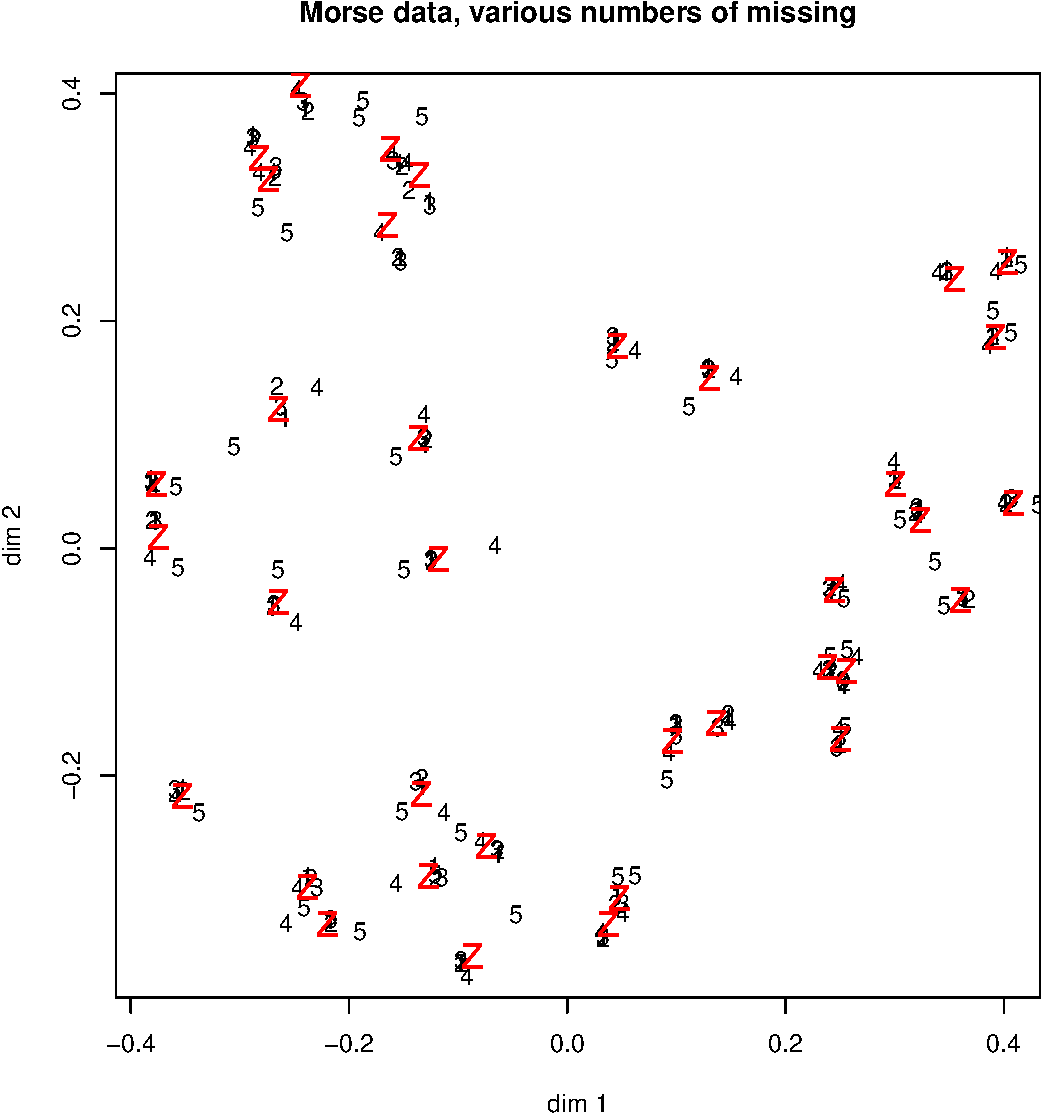
\includegraphics[keepaspectratio]{strain_files/figure-pdf/missing-1.pdf}}
\end{center}

The plot shows a stable solution. Points are labeled ``0'' for no
missing, ``1'' for 5 missing, and so on. The red points are for the
matched \(Z\) matrix. The number of iterations for 0, 5, 10, 50, 100
missing data is 0, 9, 9, 17, 23 and strain is 6.7478705, 6.6592189,
6.7039054, 6.2415359, 5.9283001.

roskam

\sectionbreak

\section{Discussion}\label{discussion}

Most MDS loss functions are of the form \begin{equation}
\sigma(X):=\sum_k w_k(f(\delta_k)-f(d_k(X)))^2\label{eq-fstress}
\end{equation} for some given function \(f\). Groenen, De Leeuw, and
Mathar (\citeproc{ref-groenen_deleeuw_mathar_C_95}{1995}) call loss
function \eqref{eq-fstress} fStress. For \(f\) equal to the identity we
have stress (Kruskal (\citeproc{ref-kruskal_64a}{1964})), for \(f\) the
square we have sstress (Takane, Young, and De Leeuw
(\citeproc{ref-takane_young_deleeuw_A_77}{1977})), and for \(f\) the
logarithm we have log-stress (Ramsay (\citeproc{ref-ramsay_77}{1977})).
If we compare \eqref{eq-fstress} and strain we see that strain is more
complicated because of the non-diagonal Kronecker weights. This makes
the usual optimal transformations in MDS, such as monotone regression in
the ordinal case, more complicated and costly. As a consequence
non-metric MDS techniques minimizing strain have not been implemented
and used to the same degree as techniques based on variations of
fStress.

On the other hand in fStress the minimization over \(X\) for given
\(\Delta\) is more costly than it is for strain, in which we simply have
to find the \(p\) largest eigenvalues and corresponding eigenvectors of
a matrix. Thus, the ALS framework, for fStress finding optimal
\(\Delta\) for fixed \(x\) is cheap and finding optimal \(X\) for fixed
\(\Delta\) is expensive. For strain it is exactly the other way around.
To put it even more sharply, in fStress finding the optimal \(X\) is
impossible, because it requires an inifinite iterative process which can
converge to a local minimum. For strain, although solving the
eigen-problem is also an infinite iterative process, it quickly gets us
as close as we want to the global minimum (for given \(Delta\), that
is).

Trosset (\citeproc{ref-trosset_02}{2002})

Trosset (\citeproc{ref-trosset_98}{1998}) discusses an implementation or
ordinal MDS uing strain. His aproach is quite different from ours,
because it does not use ALS but gradient projection. More importantly,
Trosset projects out the optimization over \(X\). He calls this
``variable reduction'', to contrast it with ``variable alternation''.
Thus his strain is a function of \(\Delta\) only, defined as
\begin{equation}
\sigma(\Delta)=\min_X\text{tr}\ (C(\Delta)- XX')^2=\sum_{r=p+1}^n\lambda_r^2(C_+(\Delta)),
\label{eq-varred}
\end{equation} where the \(\lambda_r\) are the \(n-p\) smallest
eigenvalues of its argument, and with \(C_+\) the positive definite part
of \(C\). This loss function is then minimized over \(\Delta\) by
gradient projection, constrained by the linear inequalities that impose
monotonicity. It is unclear how this compares to ALS, although we can
say that in general projecting out a set of unknowns tends to accelerate
convergence, at the cost of more complicated subproblems in each
iteration. Also, unlike ALS, gradient projection implies choosing a
step-size procedure to guarantee convergence. Projection seems
especially suitable for the additive constant problem in which
\eqref{eq-varred} is a function of a single parameter, which can be
minimized in a number of ways.

weighted strain

\sectionbreak

\section*{References}\label{references}
\addcontentsline{toc}{section}{References}

\phantomsection\label{refs}
\begin{CSLReferences}{1}{0}
\bibitem[\citeproctext]{ref-bauschke_bui_wang_18}
Bauschke, Heinz H., Minh N. Bui, and Xianfu Wang. 2018. {``{Projecting
onto the Intersection of a Cone and a Sphere}.''} \emph{SIAM Journal on
Optimization} 28: 2158--88.

\bibitem[\citeproctext]{ref-deleeuw_R_74c}
De Leeuw, Jan. 1974a. {``Approximation of a Real Symmetric Matrix by a
Positive Semidefinite Matrix of Rank r.''} Technical Memorandum
TM-74-1229-10. Murray Hill, N.J.: Bell Telephone Laboratories.
\url{https://jansweb.netlify.app/publication/deleeuw-r-74-c/deleeuw-r-74-c.pdf}.

\bibitem[\citeproctext]{ref-deleeuw_R_74b}
---------. 1974b. {``Finding a Positive Semidefinite Matrix of
Prescribed Rank r in a Nonlinear Differentiable Manifold.''} Technical
Memorandum. Murray Hill, N.J.: Bell Telephone Laboratories.
\url{https://jansweb.netlify.app/publication/deleeuw-r-74-b/deleeuw-r-74-b.pdf}.

\bibitem[\citeproctext]{ref-deleeuw_U_75a}
---------. 1975. {``{A Normalized Cone Regression Approach to
Alternating Least Squares Algorithms}.''} Department of Data Theory
FSW/RUL.
\url{https://jansweb.netlify.app/publication/deleeuw-u-75-a/deleeuw-u-75-a.pdf}.

\bibitem[\citeproctext]{ref-deleeuw_heiser_C_82}
De Leeuw, Jan, and Willem J. Heiser. 1982. {``Theory of Multidimensional
Scaling.''} In \emph{Handbook of Statistics, Volume {II}}, edited by P.
R. Krishnaiah and L. Kanal. Amsterdam, The Netherlands: North Holland
Publishing Company.

\bibitem[\citeproctext]{ref-deleeuw_hornik_mair_A_09}
De Leeuw, Jan, Kurt Hornik, and Patrick Mair. 2009. {``{Isotone
Optimization in R: Pool-Adjacent-Violators Algorithm (PAVA) and Active
Set Methods}.''} \emph{Journal of Statistical Software} 32 (5): 1--24.

\bibitem[\citeproctext]{ref-deleeuw_mair_A_09c}
De Leeuw, Jan, and Patrick Mair. 2009. {``{Multidimensional Scaling
Using Majorization: SMACOF in R}.''} \emph{Journal of Statistical
Software} 31 (3): 1--30.
\url{https://www.jstatsoft.org/article/view/v031i03}.

\bibitem[\citeproctext]{ref-gower_66}
Gower, John C. 1966. {``{Some Distance Properties of Latent Root and
Vector Methods Used in Multivariate Analysis}.''} \emph{Biometrika} 53:
325--38.

\bibitem[\citeproctext]{ref-groenen_deleeuw_mathar_C_95}
Groenen, Patrick J. F., Jan De Leeuw, and Rudolf Mathar. 1995. {``{Least
Squares Multidimensional Scaling with Transformed Distances}.''} In
\emph{{From Data to Knowledge: Theoretical and Practical Aspects of
Classification, Data Analysis and Knowledge Organization}}, edited by W.
Gaul and D. Pfeifer. Berlin, Germany: Springer Verlag.
\url{https://jansweb.netlify.app/publication/groenen-deleeuw-mathar-c-95/groenen-deleeuw-mathar-c-95.pdf}.

\bibitem[\citeproctext]{ref-groenen_giaquinto_kiers_03}
Groenen, Patrick J. F., Patrizia Giaquinto, and Henk A. L Kiers. 2003.
{``{Weighted Majorization Algorithms for Weighted Least Squares
Decomposition Models}.''} Econometric Institute Report EI 2003-09.
Econometric Institute, Erasmus University Rotterdam.
\url{https://repub.eur.nl/pub/1700}.

\bibitem[\citeproctext]{ref-jeffrey_97}
Jeffrey, David J. 1997. {``Formulae, Algorithms, and Quartic Extrema.''}
\emph{Mathematics Magazine} 70 (5): 341--48.

\bibitem[\citeproctext]{ref-keller_62}
Keller, Joseph B. 1962. {``{Factorization of Matrices by Least
Squares}.''} \emph{Biometrika} 49: 239--42.

\bibitem[\citeproctext]{ref-kiers_97}
Kiers, Henk A. L. 1997. {``{Weighted Least Squares Fitting Using
Iterative Ordinary Least Squares Algorithms}.''} \emph{Psychometrika}
62: 251--66.

\bibitem[\citeproctext]{ref-kruskal_64a}
Kruskal, Joseph B. 1964. {``{Multidimensional Scaling by Optimizing
Goodness of Fit to a Nonmetric Hypothesis}.''} \emph{Psychometrika} 29:
1--27.

\bibitem[\citeproctext]{ref-mardia_78}
Mardia, Kanti V. 1978. {``Some Properties of Classical Multidimensional
Scaling.''} \emph{Communications in Statistics - Theory and Methods} 7
(13): 1233--41.

\bibitem[\citeproctext]{ref-mullen_vanstokkum_24}
Mullen, Katherine M., and Ivo H. M. van Stokkum. 2024. \emph{{nnls: The
Lawson-Hanson algorithm for non-negative least squares (NNLS)}}.
\url{\%7Bhttps://CRAN.R-project.org/package=nnls\%7D}.

\bibitem[\citeproctext]{ref-qiu_mei_24}
Qiu, Yixuan, and Jiali Mei. 2024. \emph{{RSpectra: Solvers for
Large-Scale Eigenvalue and SVD Problems}}.
\url{https://CRAN.R-project.org/package=RSpectra}.

\bibitem[\citeproctext]{ref-r_core_team_25}
R Core Team. 2025. \emph{R: A Language and Environment for Statistical
Computing}. {Vienna, Austria}: R Foundation for Statistical Computing.
\url{https://www.R-project.org/}.

\bibitem[\citeproctext]{ref-ramsay_77}
Ramsay, James O. 1977. {``{Maximum Likelihood Estimation in
Multidimensional Scaling}.''} \emph{Psychometrika} 42: 241--66.

\bibitem[\citeproctext]{ref-rothkopf_57}
Rothkopf, Ernst Z. 1957. {``{A Measure of Stimulus Similarity and Errors
in some Paired-associate Learning}.''} \emph{Journal of Experimental
Psychology} 53: 94--101.

\bibitem[\citeproctext]{ref-saito_78}
Saito, Takayuki. 1978. {``The Problem of the Additive Constant and
Eigenvalues in Metric Multidimensional Scaling.''} \emph{Psychometrika}
43 (2): 193--201.

\bibitem[\citeproctext]{ref-schoenberg_35}
Schoenberg, Isaac J. 1935. {``{Remarks to Maurice Frechet's article: Sur
la Definition Axiomatique d'une Classe d'Espaces Vectoriels Distancies
Applicables Vectoriellement sur l'Espace de Hllbert}.''} \emph{Annals of
Mathematics} 36: 724--32.

\bibitem[\citeproctext]{ref-takane_young_deleeuw_A_77}
Takane, Yoshio, Forrest W. Young, and Jan De Leeuw. 1977. {``Nonmetric
Individual Differences in Multidimensional Scaling: An Alternating Least
Squares Method with Optimal Scaling Features.''} \emph{Psychometrika}
42: 7--67.

\bibitem[\citeproctext]{ref-torgerson_58}
Torgerson, Warren S. 1958. \emph{{Theory and Methods of Scaling}}. New
York: Wiley.

\bibitem[\citeproctext]{ref-trosset_97}
Trosset, Michael W. 1997. {``Numerical Algorithms for Multidimensional
Scaling.''} In \emph{Classification and Knowledge Organization}, edited
by Rüdiger Klar and Otto Opitz, 80--92. Springer.

\bibitem[\citeproctext]{ref-trosset_98}
---------. 1998. {``A New Formulation of the Nonmetric Strain Problem in
Multidimensional Scaling.''} \emph{Journal of Classification} 15:
15--35.

\bibitem[\citeproctext]{ref-trosset_00}
---------. 2000. {``Distance Matrix Completion by Numerical
Optimization.''} \emph{Computational Optimization and Applications} 17:
11--22.

\bibitem[\citeproctext]{ref-trosset_02}
---------. 2002. {``Extensions of Classical Multidimensional Scaling via
Variable Reduction.''} \emph{Computational Statistics} 17: 147--63.

\bibitem[\citeproctext]{ref-young_householder_38}
Young, Gale, and Alston S. Householder. 1938. {``{Discussion of a Set of
Points in Terms of Their Mutual Distances}.''} \emph{Psychometrika} 3
(19-22).

\end{CSLReferences}




\end{document}
